\documentclass[12pt,openany,a4paper]{book}
\newcommand\tabSpace[1][1cm]{\hspace*{#1}}
\usepackage{graphicx}
\usepackage{ragged2e}
\usepackage{enumitem}
\usepackage{listings}
\usepackage{amsmath}
\usepackage[subnum]{cases}
%Code coloring
\usepackage{color}
\definecolor{dkgreen}{rgb}{0,0.6,0}
\definecolor{gray}{rgb}{0.5,0.5,0.5}
\definecolor{mauve}{rgb}{0.58,0,0.82}
\lstset{
  language=C,
  xleftmargin=\parindent,
  aboveskip=3mm,
  belowskip=3mm,
  showstringspaces=false,
  columns=flexible,
  basicstyle={\small\ttfamily},
  numbers=left,
  numberstyle=\tiny\color{gray},
  keywordstyle=\color{blue},
  commentstyle=\color{dkgreen},
  stringstyle=\color{mauve},
  breaklines=true,
  breakatwhitespace=true,
  tabsize=3
}
%BibTeX referencing packages
\usepackage{lmodern}
\usepackage{hyperref}
\usepackage{breakurl}



% If you use a macro file called macros.tex :
% \input{macros}
% Note: The present document has its macros built in.

% Number subsections but not subsubsections:
\setcounter{secnumdepth}{2}
% Show subsections but not subsubsections in table of contents:
\setcounter{tocdepth}{2}

\pagestyle{headings}		% Chapter on left page, Section on right.
\raggedbottom

\setlength{\topmargin}		{-5mm}  %  25-5 = 20mm
%\setlength{\oddsidemargin}	{10mm}  % rhs page inner margin = 25+10mm
\setlength{\oddsidemargin}	{0mm}  % CHANGED THIS BECAUSE I DIDNT LIKE IT
\setlength{\evensidemargin}	{0mm}   % lhs page outer margin = 25mm
\setlength{\textwidth}		{150mm} % 35 + 150 + 25 = 210mm
\setlength{\textheight}		{240mm} % 

\renewcommand{\baselinestretch}{1.2}	% Looks like 1.5 spacing.

% Stop figure/tables smaller than 3/4 page from appearing alone on a page:
\renewcommand{\textfraction}{0.25}
\renewcommand{\topfraction}{0.75}
\renewcommand{\bottomfraction}{0.75}
\renewcommand{\floatpagefraction}{0.75}

% THEOREM-LIKE ENVIRONMENTS:
\newtheorem{defn}	{Definition}	% cf. \dfn for cross-referencing
\newtheorem{theorem}	{Theorem}	% cf. \thrm for cross-referencing
\newtheorem{lemma}	{Lemma}		% cf. \lem for cross-referencing

% AIDS TO CROSS-REFERENCING (All take a label as argument):
\newcommand{\eref}[1] {(\ref{#1})}		% (...)
\newcommand{\eq}[1]   {Equation~(\ref{#1})}		% Eq.~(...)
\newcommand{\eqs}[2]  {Eqs.~(\ref{#1}) and~(\ref{#2})}
\newcommand{\dfn}[1]  {Definition~\ref{#1}}	% Definition~...
\newcommand{\thrm}[1] {Theorem~\ref{#1}}	% Theorem~...
\newcommand{\lem}[1]  {Lemma~\ref{#1}}		% Lemma~...
\newcommand{\fig}[1]  {Figure~\ref{#1}}		% Fig.~...
\newcommand{\tab}[1]  {Table~\ref{#1}}		% Table~...
\newcommand{\chap}[1] {Chapter~\ref{#1}}	% Chapter~...
\newcommand{\secn}[1] {Section~\ref{#1}}	% Section~...
\newcommand{\ssec}[1] {Subsection~\ref{#1}}	% Subsection~...

% AIDS TO FORMATTING:
\newcommand{\teq}[1]	{\mbox{$#1$}}	% in-Text EQuation (unbreakable)
\newcommand{\qed}	{\hspace*{\fill}$\bullet$}	% end of proof

% MATHEMATICAL TEMPLATES:
% Text or math mode:
\newcommand{\half}	{\ensuremath{\frac{1}{2}}}	% one-half
\newcommand{\halftxt}	{\mbox{$\frac{1}{2}$}}	  	% one-half, small
% Math mode only:
% N.B. Parentheses are ROUND; brackets are SQUARE!
\newcommand{\oneon}[1]	{\frac{1}{#1}}		  % reciprocal
\newcommand{\pow}[2]	{\left({#1}\right)^{#2}}  % Parenthesized pOWer
\newcommand{\bow}[2]	{\left[{#1}\right]^{#2}}  % Bracketed pOWer
\newcommand{\evalat}[2]	{\left.{#1}\right|_{#2}}  % EVALuated AT with bar
\newcommand{\bevalat}[2]{\left[{#1}\right]_{#2}}  % Bracketed EVALuated AT
% Total derivatives:
\newcommand{\sdd}[2]	{\frac{d{#1}}{d{#2}}}		    % Short
\newcommand{\sqdd}[2]	{\frac{d^2{#1}}{d{#2}^2}}	    % 2nd ("SQuared")
\newcommand{\ldd}[2]	{\frac{d}{d{#1}}\left({#2}\right)}  % Long paren'ed
\newcommand{\bdd}[2]	{\frac{d}{d{#2}}\left[{#2}\right]}  % long Bracketed
% Partial derivatives (same sequence as for total derivatives):
\newcommand{\sdada}[2]	{\frac{\partial {#1}}{\partial {#2}}}
\newcommand{\sqdada}[2]	{\frac{\partial ^{2}{#1}}{\partial {#2}^{2}}}
\newcommand{\ldada}[2]	{\frac{\partial}{\partial {#1}}\left({#2}\right)}
\newcommand{\bdada}[2]	{\frac{\partial}{\partial {#1}}\left[{#2}\right]}
\newcommand{\da}	{\partial}

% ORDINAL NUMBERS:
\newcommand{\ith}	{\ensuremath{i^{\rm th}}}
\newcommand{\jth}	{\ensuremath{j^{\rm th}}}
\newcommand{\kth}	{\ensuremath{k^{\rm th}}}
\newcommand{\lth}	{\ensuremath{l^{\rm th}}}
\newcommand{\mth}	{\ensuremath{m^{\rm th}}}
\newcommand{\nth}	{\ensuremath{n^{\rm th}}}

% SINUSOIDAL TIME AND SPACE-DEPENDENCY FACTORS:
\newcommand{\ejot}	{\ensuremath{e^{j\omega t}}}
\newcommand{\emjot}	{\ensuremath{e^{-j\omega t}}}

% UNITS (TEXT OR MATH MODE, WITH LEADING PADDING SPACE IF APPLICABLE):
% NB: These have not been tested since being modified for LaTeX2e.
\newcommand{\pack}	{\hspace{-0.08em}}
\newcommand{\Pack}	{\hspace{-0.12em}}
\newcommand{\mA}	{\ensuremath{\rm\,m\pack A}}
\newcommand{\dB}	{\ensuremath{\rm\,d\pack B}}
\newcommand{\dBm}	{\ensuremath{\rm\,d\pack B\pack m}}
\newcommand{\dBW}	{\ensuremath{\rm\,d\pack B\Pack W}}
\newcommand{\uF}	{\ensuremath{\rm\,\mu\pack F}}
\newcommand{\pF}	{\ensuremath{\rm\,p\pack F}}
\newcommand{\nF}	{\ensuremath{\rm\,n\pack F}}
\newcommand{\uH}	{\ensuremath{\rm\,\mu\pack H}}
\newcommand{\mH}	{\ensuremath{\rm\,m\pack H}}
\newcommand{\Hz}	{\ensuremath{\rm\,H\pack z}}
\newcommand{\kHz}	{\ensuremath{\rm\,k\pack H\pack z}}
\newcommand{\MHz}	{\ensuremath{\rm\,M\pack H\pack z}}
\newcommand{\GHz}	{\ensuremath{\rm\,G\pack H\pack z}}
\newcommand{\J}		{\ensuremath{\rm\,J}}
\newcommand{\kg}	{\ensuremath{\rm\,k\pack g}}
\newcommand{\K}		{\ensuremath{\rm\,K}}
\newcommand{\m}		{\ensuremath{\rm\,m}}
\newcommand{\cm}	{\ensuremath{\rm\,cm}}
\newcommand{\km}	{\ensuremath{\rm\,k\pack m}}
\newcommand{\mm}	{\ensuremath{\rm\,m\pack m}}
\newcommand{\nm}	{\ensuremath{\rm\,n\pack m}}
\newcommand{\um}	{\ensuremath{\rm\,\mu m}}
\newcommand{\Np}	{\ensuremath{\rm\,N\pack p}}
\newcommand{\s}		{\ensuremath{\rm\,s}}
\newcommand{\ms}	{\ensuremath{\rm\,m\pack s}}
\newcommand{\us}	{\ensuremath{\rm\,\mu s}}
\newcommand{\V}		{\ensuremath{\rm\,V}}
\newcommand{\mV}	{\ensuremath{\rm\,m\Pack V}}
\newcommand{\W}		{\ensuremath{\rm\,W}}
\newcommand{\mW}	{\ensuremath{\rm\,m\Pack W}}
\newcommand{\ohm}	{\ensuremath{\rm\,\Omega}}
\newcommand{\kohm}	{\ensuremath{\rm\,k\Omega}}
\newcommand{\Mohm}	{\ensuremath{\rm\,M\Omega}}
\newcommand{\degs}	{\ensuremath{\rm^{\circ}}}






% LaTeX run-time type-in command:
%
% \typein{Enter \protect\includeonly{...} command (or just type RETURN):}
%
% Uncommenting this command makes LaTeX prompt you for the \includeonly
% list.  At the prompt
%
%	\@typein=
%
% you type
%
%	\includeonly{chap1,chap2}
%
% to include the files chap1.tex and chap2.tex and omit any others.
% To include every \include file, just hit RETURN.
% If you are running LaTeX from xtexsh, you may need to click the mouse
% in the LaTeX window to position the cursor at the \@typein prompt.



\begin{document}

\frontmatter
% By default, frontmatter has Roman page-numbering (i,ii,...).

\begin{titlepage}
	\centering
	
\includegraphics[width=10cm]{UQLogo.png}
\renewcommand{\baselinestretch}{1.0}
\begin{center}
\vspace*{15mm}
\Huge\bf
		RF Switching\\ system for\\ Biomedical Radar systems \\
\vspace{20mm}
\large\sl
		by\\
		Matt Pascoe
		\medskip\\
\rm
		School of Information Technology and Electrical Engineering,\\
		The University of Queensland.\\
\vspace{30mm}
		Submitted for the degree of\\
		Bachelor of Engineering
		\smallskip\\
\normalsize
		in the field of Electrical Engineering 
		\medskip\\
\large
		\today		
\end{center}
\end{titlepage}
\newpage



\begin{flushright}
	1/55 Bellevue Terrace\\
	St Lucia, QLD  4067\\
	Tel.\ (04) 1313 1840\\
	\medskip
	\today
\end{flushright}
\begin{flushleft}
  Prof Paul Strooper\\
  Head of School\\
  School of Information Technology and Electrical Engineering\\
  The University of Queensland\\
  St Lucia, Q 4072\\
  \bigskip\bigskip
  Dear Professor Strooper,
\end{flushleft}
In accordance with the requirements of the degree of Bachelor of
Engineering in the division of Electrical Engineering I present the
following thesis entitled ``RF Switching System for Biomedical Radar 
Systems''.  This work was performed under the supervision of
Dr. Konstanty Bialkowski. \\
I declare that the work submitted in this thesis is my own, except as
acknowledged in the text and footnotes, and has not been previously
submitted for a degree at The University of Queensland or any other
institution.

\begin{flushright}
	Yours sincerely,\\
	\medskip
	\emph{Matt Pascoe}\\
	\medskip
	Matt Pascoe.
\end{flushright}
\newpage


%
%\chapter{Acknowledgments}
%%Acknowledge your supervisor, preferably with a few short and specific
%%statements about his/her contribution to the content and direction of
%%the project.  If you collaborated with another student, acknowledge
%%your partner's contribution, including any parts of the thesis of
%%which s/he was the principal author or co-author; this information can
%%be duplicated in footnotes to the chapters or sections to which your
%%partner has contributed.  Briefly describe any assistance that you
%%received from technical or administrative staff.  Support of family
%%and friends may also be acknowledged, but avoid sentimentality---or
%%hide it in the dedication.
%I would like to thank John Kohlbach and the staff at the ETSG for providing me with access to ... . I would also like to thank Dr. Konstanty Bialkowski for giving me the opportunity to work on an interesting subject, ... and providing support on the project.
%\newpage












%---------------------------------------------------------------------------------
\chapter{Abstract}
This document is a skeleton thesis for 4th-year students.  The
printable versions (\texttt{skel.dvi, skel.ps, skel.pdf})
show the structure of a typical thesis with some notes on the content
and purpose of each part.  The notes are meant to be informative but
not necessarily illustrative; for example, this paragraph is not
really an abstract, because it contains information not found
elsewhere in the document.  The \LaTeXe\ source file
(\texttt{skel.tex}) contains some non-printing comments giving
additional information for students who wish to typeset their theses
in \LaTeX.  You can download the source, edit out the unwanted
material, insert your own frontmatter and bibliographic entries, and
in-line or \verb+\include{}+ your own chapter files.  Of course the
content of a particular thesis will influence the form to a large
extent.  Hence this document should not be seen as an attempt to force
every thesis into the same mold.  If in doubt about the structure of
your thesis, seek advice from your supervisor.
\newpage

%---------------------------------------------------------------------------------




\tableofcontents

%Abbreviations

\listoffigures
\addcontentsline{toc}{chapter}{List of Figures}

\listoftables
\addcontentsline{toc}{chapter}{List of Tables}



% If file los.tex begins with ``\chapter{List of Symbols}'':
% \include{los}

\newpage


\mainmatter










% -------------------------------------------------------------------------------
%TODO : add references for the 5 \cites in this section
%
%TODO : review section to make more appropriate for final submission

%TODO : look for journal papers about people using biomedical radar devices and how they take a long time, if faster switching is used then they would get better speeds.

\chapter{Introduction}
\section{Background}
\justify
There has been a growing demand for the development of wireless systems, to meet the increasing demands of consumers. In order to meet this demand researchers have looked to software defined radio's (SDR); this interest in SDR is due to the ease and simplicity for the development and implementation in various applications. This rise in interest has led to a large spike in development of SDR, which is resulting in a broadened application for SDR. \cite{ref1} \\
SDR's are being applied in a variety of different scenarios, but this thesis focuses primarily on the development of a switching system to complement the research done using SDR as a tool for medical imaging. The use of SDR in microwave imaging has provided an alternative diagnostic tool that presents significant benefits of current technology, primarily because of its low cost, portability, non-invasiveness and uses non-ionization radiation. This allows the system to be compact and suitable for medical application in the field. \cite{ref2} \cite{ref3} \\
As the demand for faster wireless systems increases, so does the interest in researching the application of using multiple antenna wireless links for digital communication; using multiple antennas introduces a greater range of possibilities by increasing the speed of the networks traffic \cite{ref4}. To accommodate for the control of multiple radio frequency (RF) front ends the communication system will require a RF switching system; there are two primary categories for RF and microwave switches, electromechanical relay (EMR) and solid-state relay (SSR). \\
There are advantages and disadvantages in use either, SSR's are available in smaller packages and have a higher switching speed but are restricted to single pole, EMR's have a lower isolation loss but are have slower speed due to their physical construction. SSR don't have a wearable switching mechanism while EMR do, making them impractical in scenarios which require large amounts of switching \cite{ref5}. Therefore, this thesis will primarily focus on utilising SSR's as opposed to EMR's, to meet the high speed requirements while maintaining a low cost and compact design. \\
This thesis project looks into the development of an RF switching system to allow an RF front end to be connected to a large number of antennas or sensors, by developing a RF switch matrix that provides a high speed switching on multiple antennas. The results obtained from this will facilitate and support the expansion in the current development of biomedical RF imaging systems as well as future projects.



%TODO : talk about how "speed is relevant to the VNA, so the switches dont limit the overall speed of the device.
\section{Aims/Objectives}
This thesis aims to evaluate the current available designs and products to develop a low-cost and portable RF switch matrix. \newline
The primary objective are to complete the following tasks: \\[-0.8cm]
\begin{itemize}
	\setlength\itemsep{-0.5em}
	\item Evaluate and Design a RF Switch matrix
	\item Develop and Construct the RF Switch matrix
	\item Finalise and construct a housing for the switch matrix
\end{itemize}




\section{Thesis Structure}
\textbf{Chapter 2} investigates the prior technology available that can be adapted or utilised in order to assist in the development of RF switching system. \newline
\textbf{Chapter 3} defines the relevant theory that is required to understand the topics discussed in this thesis. \newline
\textbf{Chapter 4} looks into the analysis and development of RF switches. \newline
\textbf{Chapter 5} depicts the flow of the project, starting from the thesis's definition and following it through the solution, design, simulation, implementation and results. \newline
\textbf{Chapter 6} contains performance results of the RF switch matrix, and the RF switch matrix's characteristics. \newline
\textbf{Chapter 7} discusses the performance of the produced switch matrix and future work.  
\newline




\section{Expected Contribution}
The thesis will look at developing a low-cost RF switch matrix capable of providing a $2$ input, $16$ output switching matrix. It should reveal the possibility of developing switch matrix's that are better suited to low-cost, portable projects in contrast to commercially available switches.\newline
This thesis is expected to produce a proprietary switch matrix that can enable the further development of low-power RF development in biomedical and radar applications.


%---------------------------------------------------------------------------------












%---------------------------------------------------------------------------------

\chapter{Literature review}
\section{Prior Art}
This chapter looks into the currently available designs used for high speed RF switching as well as relevant theory that has and is being completed in the field.


%TODO : Look into mechanical motion technology in rf imaging techniques???
\subsection{Currently Available Technology}


\subsection{Previous designs}
In order to develop the PCB 




\section{Software Defined Radio}
The application of the RF switching system this thesis looks a developing, is to provide an RF front end such as a software defined radio (SDR) or Vector Network Analyser (VNA) with the ability to communicate multiple antennas or sensors. An SDR is a radio that is partially or entirely controlled by software in the physical layer in the Open Systems Interconnection (OSI) model. The OSI model is used to describe the subsystems of a communication system, where the physical layer represents the data. This allows for the software or firmware to be adjusted resulting in the change the carrier frequency, data rate, modulation, coding, etc. without having the reconstruct the hardware of the radio [6]. This project doesn't look into the control of an SDR, instead focuses on interfacing the switching system with the SDR. It is expected that the SDR will have an impedance of $50\ohm$ which is common of most SDR technology or a less common impedance of $75\ohm$ [7].

\subsection{Analysing SDR Signals}

\subsection{Radar Signal Analysis}



\section{Microwave Theory}
To design and develop microwave circuits a fundamental understanding of how microwaves operate and ... in ... is required

\subsection{Transmission Line Theory}
A transmission line is a medium that transfers electromagnetic energy along its path, an example can be seen in \fig{fig:tline}. Transmission lines will form the primary basis of this thesis since it will be primary medium for the signal travelling through the RF switching system. It is crucial to ensure that the transmission line matches the source and antenna; otherwise it can cause the power to be reflected back. \newline
\begin{figure}[h]
	\centering
    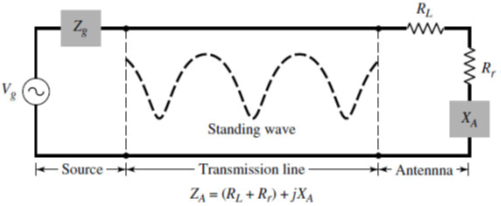
\includegraphics[width=0.8\textwidth]{tline.png}
	\caption{Transmission line Thevenin equivalent of antenna and transmitter}
	\label{fig:tline}
\end{figure} 
To prevent this reflection, the impedances at each end must be matched to the transmission lines characteristic impedance. This can be done through L-section matching, stepped transmission lines or filters.  \\[0.1cm]
L-section is a method used for matching transmission lines; this involves using a capacitor and inductor in a series and parallel combination to match the load. Stepped transmission lines provides impedance matching for lumped elements. Finally, filters can also be used for impedance matching; they are typically used to provide an adjustable match for the circuit over different frequencies. By inserting a filter that is a perfect match for the transmission line at a known frequency [9]. This theory will be considered when evaluating the design for the development boards and if required the PCB so they are perfectly matched to reduce any unnecessary losses in the system.

\subsection{Scattering Parameters}
Scattering parameters (S-Parameters) are a matrix that describes the behaviour of linear electrical networks; this matrix is used over a broad range of disciplines of electrical engineering but is particularly useful in microwave engineering.
Since the RF switching system this thesis is designing will not generating its own signal or provide any RF front end's; even though the system is switching, it will always have a single input and single output. Therefore, this design can be simplified to be a 2-port network, as shown in Figure 2.\\[0.1cm]
%figure
2-port networks are most commonly used and can easily be adapted to systems that are more complex, Figure 2 shows a simple diagram of a 2-port network and Equation 1 shows the matrix and equations given for the network [9].

\subsection{System Losses}










\section{RF Switches}
This thesis topic looks into the development of a RF switching system, this will be done by utilising RF and microwave switches to create an RF switching matrix. An RF switch matrix are used to route RF signals from an input to an output.
There are several different types of switching matrix's, there is multiple input multiple output (MIMO), multiple input single output (MISO), single input multiple output (SIMO) and single input single output (SISO) [12]. For this project we are looking at controlling multiple outputs with a single input, so will be implementing a SIMO RF switching matrix.

\subsection{Switch Architecture}


\subsection{Switch Topologies}
When constructing a RF switch there are two typical topologies, these are multiplexers and general purpose relays; examples can be seen in Figure 3. General purpose relays are commonly a SPDT or SDnT relay's that are used for routing a signal between multiple paths. Multiplexers are devices that route a single input to multiple outputs or vice versa, they are commonly built from multiple SPDT relays but have a greater inherited insertion loss from this configuration [13]. 
%IMAGE
Looking at Figure 3 (b) it can be assumed that there will be losses through each path it takes, insertion loses through first switch, first cable/track, second switch, etc. Therefore, it is ideal to develop a topology as close to Figure 3 (a) to ensure there is little loss through multiple cascaded switches and cable/tracks. This thesis will be looking into designing a 1x12 SIMO multiplexer, similar to the design in Figure 3 (b) to provide the available ports as well as a consistent loss through the system.




\section{Substrate Selection}
%talk about different available substrates, pros/cons ->how they effect high freq. ->cost
%discuss which are most suitable for this project. MAKE disciosion
There are various substrates that are available for developing the RF switching matrix. Four key substrates were looked at these include:
\begin{itemize} [noitemsep,topsep=0pt]
  \item FR-4
  \item Epoxy
\end{itemize}
Table \ref{tab:substrate} contains the characteristics of these four substrates that are utilised to calculate the dimensions of the RF tracks. 
When designing PCB's for 



%TODO : Replace 'track' with 'transmission line'
\section{RF Track Design}
%talk about; microstrip, stripline, coplanar. design techniques, 
For designing the RF tracks on the PCB there are three primary options available
\begin{itemize}[noitemsep,topsep=0.5pt]
	\item Micro-strip
	\item Coplanar Wave-guide, and
	\item Strip-line
\end{itemize}
RF tracks provide ...\\
For designing the tracks we need to consider:
\begin{align}
\lambda&= \frac{c}{f\sqrt{\epsilon_{eff}}} \label{eq:lam} \\
\theta &= \frac{2 \pi}{\lambda} \label{eq:phase}
\end{align}
We need to consider the Figure \ref{eq:lam} and \ref{eq:phase} as these are the fundamentals for designing any type of track. To determine which track is best suited this thesis will look at each available option.\newline
%------
These equations are used for the approximate design of RF tracks, in order to obtain a more precise design which consider a wider range of variables dedicated software is  used to further verify the design of the tracks.
%REFERENCE

\subsection{Micro-strip}
Microstrip RF tracks are the most common RF transmission line currently used in practice. %NEED TO CITE THIS!!!!
%---------------------
% need to talk about microstrip in general
%----------------------
\fig{fig:microdiag} presents a typical microstrip which has been labelled the critical dimensions of this transmission line. \newline
\begin{figure}[h]
	\centering
    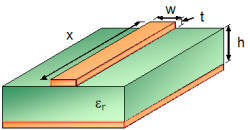
\includegraphics[width=0.65\textwidth]{microdiag.jpg}
	\caption{Microstrip diagram}
	\label{fig:microdiag}
\end{figure} 
We are able to calculate the dimensions shown in \fig{fig:microdiag} by using the following:
\begin{align}
W&=\frac{t}{\pi} \left[ ln \left( \frac{2h}{t} \right) +1 \right] \\
H&=h-2t 
\end{align}
\begin{numcases}{\epsilon_{eff}=}
	\frac{\epsilon_r+1}{2} + \frac{\epsilon-1}{2} \left[ \frac{1}{\sqrt{1+\frac{12H}{W}}} +0.04 \left(1- \frac{W}{H} \right)^2 \right] &$when \left( \frac{W}{H} \right) < 1$  \label{eq:epsh<1} \\
	\frac{\epsilon+1}{2}+ \frac{\epsilon-1}{2\sqrt{1+\frac{12H}{W}}} & $when \left( \frac{W}{H} \right) > 1$  \label{eq:epsh>1}
\end{numcases}
\begin{numcases}{Z_0=}
   \frac{60}{\sqrt{\epsilon_{eff}}} \cdot ln\left( \frac{8H}{W}+\frac{W}{4H} \right), & $when \left( \frac{W}{H} \right) < 1$  \label{eq:microh<1} \\
   \frac{120 \pi}{\sqrt{\epsilon_{eff}} \cdot \left[ \frac{W}{H}+1.393+\frac{2}{3}ln \left(\frac{W}{H}+1.444 \right) \right]}, & $when \left( \frac{W}{H} \right) > 1$ \label{eq:microh>1}
\end{numcases}
In order to calculate the dimensions of the micro-strip track we are required to make key decisions for the design. By selecting the frequency range, impedance, phase shift substrate and track thickness we are able to determine the dimensions for the track. \newline
We are able to determine the width ($W$) and length($X$) of the track by selecting a substrate determining the dielectric constant ($\epsilon_{eff}$), copper thickness ($t$) and height($H$). We can set the 


%why we should use this, characteristics, limitations ect.


\subsection{Strip-line}
Stripline RF tracks are ... \newline

We are able to caluclate the dimensions shown in Figure 3.2

\subsection{Coplanar Wave-guide}
C












%Physical Enclosure & track losses
\section{Radiation Emission}


\subsection{Picket Fencing Technique}


\subsection{Shielding}


%---------------------------------------------------------------------------------








%---------------------------------------------------------------------------------
\chapter{RF Switch Evaluation}
In this chapter the design of discrete RF switches is evaluated in comparaison to commercially available switches. This chapter will look into the design and simulations of SPDT, SP4T and SP8T RF switches within the frequency range of 100MHz-4GHz to gain a better understanding of RF switch functionality and variants.
 
\section{RF Switch Design}
There are two 


\subsection{PIN Diode}


\subsection{FET}

\section{Topologies}



\section{Available RF Switches}

%---------------------------------------------------------------------------------
 






%---------------------------------------------------------------------------------
\chapter{Methodology}
%the steps needed to be taken
%characterisation, analysis, pcb design, pcb manufacture, testing/evaluation, redesign or implementation
For this Thesis the design has been broken into five primary sections:\\[-0.8cm]
\begin{itemize}
	\setlength\itemsep{-0.5em}
	\item Evaluation of RF switches
	\item Design a switch matrix
	\item Develop PCB design
	\item Evaluate the RF switch matrix
	\item Construction of matrix enclosure
\end{itemize}
This chapter will cover the progression of the design and development of the RF switch matrix for the thesis.




\section{Evaluation}

\subsection{Evaluation Boards}
We currently have $3$ boards available 



The three available evaluation boards we investigated using a MODELNUMBER VNA; each switch was wired so that the input is connected to the output, while all other ports were $50\ohm$ terminated. The switch was powered and the controls set to allow the signal to proprigate down the open path, then changed the state to have a closed path; this was conducted for each evaluation board. The results were exported to a \textit{.s2p} file to be analysed using ADS, and the results can be seen in Figure's \ref{fig:res:}, \ref{fig:res:} \& \ref{fig:res:}. 
%Insert Images
These simulations 



\subsection{RF Switches}



\subsection{Transmission Line Design}








\section{Design}
For the design of the RF switch matrix, several key design citerias were identified to be required for the final product of the switch matrix. These are:
\begin{itemize}
	\setlength\itemsep{-0.5em}
	\item Two RF inputs
	\item Sixteen RF outputs
	\item Maximum path loss of $3$dB
	\item Power-able from low-power device (such as USB)
	\item Input and output are $50\ohm$
\end{itemize}
In order to meet these specifications 

Using the evaluated RF switches two separate designs are developed , 







\section{Development}
This section looks at the development of the RF switch matrix.
\subsection{PCB Development}


One of the key design parameters is for developing a portable device, this requires the switch matrix to be as small as possible. To determine the best solution ADS's LineCalc is used to % 



\subsection{RF Switch Development}





\section{Physical Construction}




\section{Micro-controller Development}
%TODO : Discus key design requirements for the microcontroller
%TODO : device selection




%TODO : Flow chart, block diagram
\subsection{Design}



\subsection{Evaluation}


%---------------------------------------------------------------------------------









%---------------------------------------------------------------------------------
\chapter{Verification}

\section{Individual Board's}
This section looks at the results obtain from each of the 


\section{RF Switch Matrix}

\subsection{Losses}

\subsection{Speed}

\subsection{Power Requirements \& Control}

%---------------------------------------------------------------------------------






%---------------------------------------------------------------------------------
\chapter{Discussion}
\section{Problems}

\subsection{Resource Availability}


\section{Objective Fulfilment}



\section{Contributions}





%---------------------------------------------------------------------------------









%---------------------------------------------------------------------------------
\chapter{Conclusions and Future Work}

\section{Conclusion}


%TODO : Intergrate an SDR into the switch matrix, replacing the microcontroller allowing for more precise control over switches
\section{Future Work}



%---------------------------------------------------------------------------------




\appendix
\addcontentsline{toc}{part}{Appendices}


\newpage
\chapter{PCB Design}
\section{Design 1}	\label{sec:pcb_design1}

\section{Design 2}	\label{sec:pcb_design2}

\section{Design 3}	\label{sec:pcb_design3}

\section{Output Design 1}	\label{sec:pcb_outdesign1}

\section{Output Design 2}	\label{sec:pcb_outdesign2}

\section{Output Design 3}	\label{sec:pcb_outdesign3}
















\chapter{Substrate Parameters}
The following tables contain the parameters and details for the substrates investigated in this thesis. \newline
\begin{table}[!htbp]
\centering
\begin{tabular}{|c|c|}
\hline
Parameter 	& Value \\
\hline
Er 	& 4.7 	\\
Mur 	& 1 \\
H 	& even 	\\
\hline
\end{tabular}
\label{tab:substrate}
\caption{\sl Parameters for simulation of FR-4 substrate}
\end{table}

\chapter{Bill of Materials}
In order to construct the design of the Switching Matrix we require the following components, a Bill of Materials has been constructed and can be seen in \tab{tab:bom}.
\begin{table}[!htbp]
\centering
\begin{tabular}{|c|c|c|c|c|c|c|}
\hline
Name & Description & Digikey Part no. & Min Order no. & Price & Quantity & Total \\
\hline
& & & & & & \\
\hline
\multicolumn{7}{c}{} \\
\hline
\multicolumn{5}{|c}{} & \textbf{Total}: & \$$100$\\
\hline
\end{tabular}
\label{tab:bom}
\caption{\sl Bill of Materials}
\end{table}











\chapter{RF Switch Controls}







\chapter{Companion disk}

If you wish to make some computer files available to your examiners,
you can list and describe the files here.  The files can be supplied
on a disk and inserted in a pocket fixed to the inside back cover.

The disk will not be needed if you can specify a URL from which the
files can be downloaded.

\cleardoublepage









\addcontentsline{toc}{section}{\protect\numberline{}Bibliography}
\bibliographystyle{IEEEtran}
\bibliography{ref}

\end{document}